\let\negmedspace\undefined
\let\negthickspace\undefined
\documentclass[journal,12pt,twocolumn]{IEEEtran}
\usepackage{cite}
\usepackage{amsmath,amssymb,amsfonts,amsthm}
\usepackage{algorithmic}
\usepackage{graphicx}
\usepackage{textcomp}
\usepackage{xcolor}
\usepackage{txfonts}
\usepackage{listings}
\usepackage{enumitem}
\usepackage{mathtools}
\usepackage{gensymb}
\usepackage{comment}
\usepackage[breaklinks=true]{hyperref}
\usepackage{tkz-euclide} 
\usepackage{listings}
\usepackage{gvv}                                        
\def\inputGnumericTable{}                                 
\usepackage[latin1]{inputenc}                                
\usepackage{color}                                            
\usepackage{array}                                            
\usepackage{longtable}                                       
\usepackage{calc}                                             
\usepackage{multirow}                                         
\usepackage{hhline}                                           
\usepackage{ifthen}                                           
\usepackage{lscape}

\newtheorem{theorem}{Theorem}[section]
\newtheorem{problem}{Problem}
\newtheorem{proposition}{Proposition}[section]
\newtheorem{lemma}{Lemma}[section]
\newtheorem{corollary}[theorem]{Corollary}
\newtheorem{example}{Example}[section]
\newtheorem{definition}[problem]{Definition}
\newcommand{\BEQA}{\begin{eqnarray}}
\newcommand{\EEQA}{\end{eqnarray}}
\newcommand{\define}{\stackrel{\triangle}{=}}
\theoremstyle{remark}
\newtheorem{rem}{Remark}
\begin{document}
\bibliographystyle{IEEEtran}
\vspace{3cm}
\title{10.5.3}
\author{EE23BTECH11027 - K RAHUL$^{*}$% <-this % stops a space
}
\maketitle
\newpage
\bigskip
\renewcommand{\thefigure}{\theenumi}
\renewcommand{\thetable}{\theenumi}
QUESTION:\\
The first and the last terms of an AP are 17 and 350 respectively. If the common difference
is 9, how many terms are there and what is their sum?\\
\bigskip \bigskip


SOLUTION:
\begin{table}[ht]
\setlength{\arrayrulewidth}{0.3mm}
\setlength{\tabcolsep}{15pt}
\renewcommand{\arraystretch}{1.5}

table 1\\

\begin{tabular}{ |p{1cm}|p{3cm}|p{1cm}| }
\hline
\multicolumn{3}{|c|}{Parameters in expression}\\
\hline
Symbol & Description & Value\\
\hline
n & The nth term of series & To be computed\\
\hline
$a_n$ & nth term of series & 350\\
\hline
$a_0$ & 0th term of series & 17 \\
\hline
d & Common difference of AP & 9\\
\hline
\end{tabular}


\end{table}
\begin{align}
x(n) &= (x(0) + nd)u(n)\\
x(l)&=(17+9l)u(l)
\end{align}

Thus,
\begin{align}{l = 37}\end{align}
Using \eqref{eq:APSum},
\begin{align}
	X(z) &= \frac{(17-8z^{-1})}{{(1-z^{-1})}^2},
\quad \abs{z} > \abs{1}\\
y(n) &= x(n) * u(n)\\
\implies Y(z) &= X(z)U(z)\\
&= \frac{(17-8z^{-1})}{(1-z^{-1})^{3}}\end{align}
\bigskip
Using contour integral to find Z transform, we get
\begin{align}
    y(37) &= \frac{1}{2\pi j} \oint _C Y(z)z^{36}dz\\
    &= \frac{1}{2\pi j} \oint _C \frac{(17-8z^{-1})}{(1-z^{-1})^{3}}z^{36}dz
\end{align}
Now, using Cauchy's residual theorem and observing the fact that 3 repeated poles exist at z = 1, 
\begin{align}
    R &= \frac{1}{(k-1)!}\lim_{z \to c}\frac{d^{k-1}}{dz^{k-1}}((z-c)^kf(z))\\
    &= \frac{1}{2!}\lim_{z \to 1}\frac{d^{k-1}}{dz^{k-1}}((z-1)^3\frac{(17-8z^{-1})}{(1-z^{-1})^{3}}z^{36})\\
    &=\frac{1}{2}\lim_{z \to 1}\frac{d^2}{dz^2}(17z^{39} - 8z^{38})\\
    &= 6973
\end{align}
\begin{figure}[h]
    %\caption{Stem Plot of $x(n)$ v/s n}
    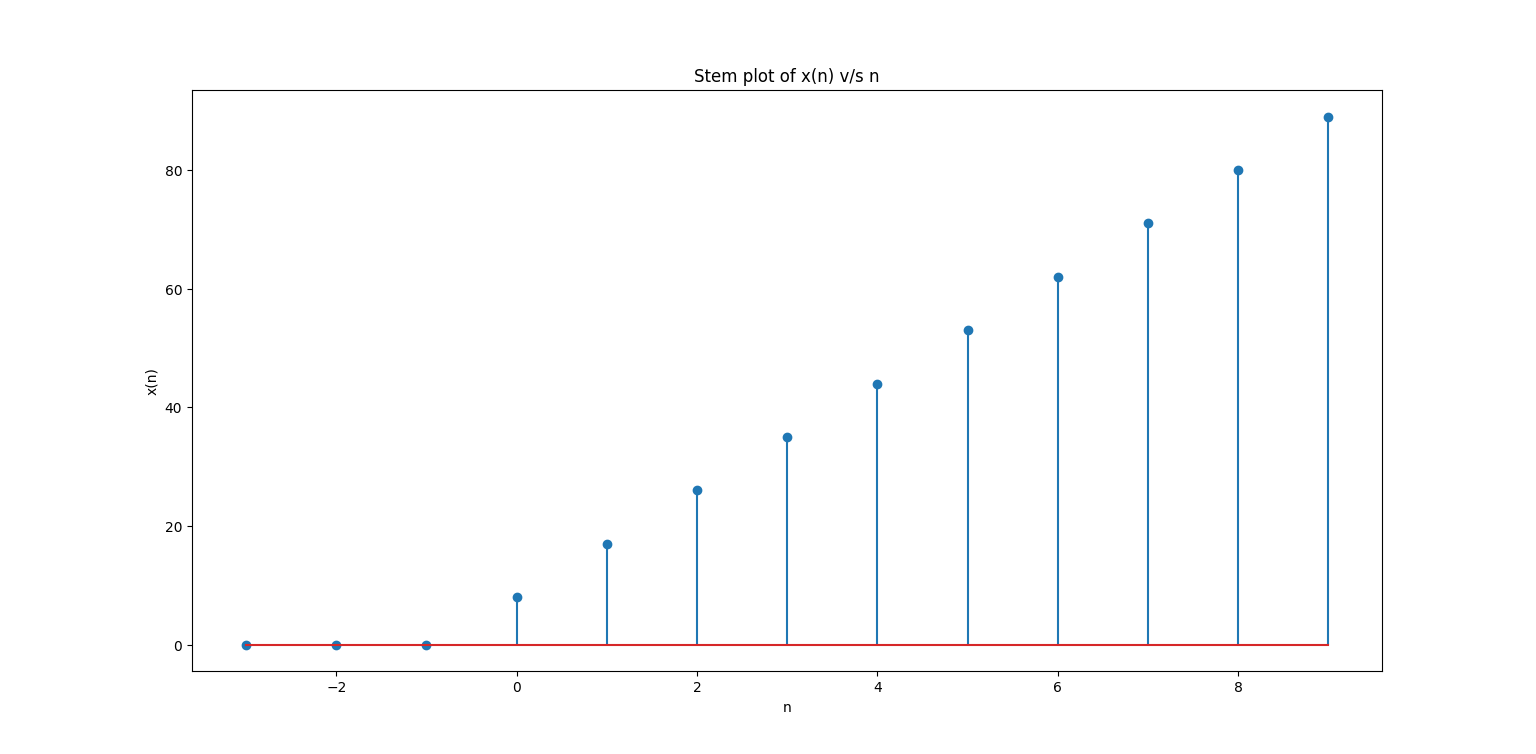
\includegraphics[width=0.5\textwidth]{figs/x(n)_plot.png}\label{fig:stem-plot}
    \caption{Stem Plot of $x(n)$ v/s n}
\end{figure}
\end{document}
